\section{Introducción: Problemática de usar librerías web en la \jvm}
\label{sec:intro}

\subsection{Desarrollo de sistemas web en la \jvm}
\label{subsec:intro:jvm_dev}

La creciente popularidad de los lenguajes que corren sobre la Máquina Virtual 
de Java (\jvm)\footnote{
	La \jvm es una parte fundamental de la plataforma del lenguaje Java,
	creada originalmente por \emph{Sun Microsystems}. La maquina virtual crea 
	una capa de abstracción entre el sistema operativo y el código Java 
	compilado (\bytecode). De esta forma, el código \java puede ser compilado a 
	\bytecode una sola vez, y correrse en cualquier sistema que cuente con una 
	\jvm.
}, y los cambios por los que ha transitado el desarrollo de 
soluciones empresariales a lo largo del tiempo hacen de esta plataforma una de 
las principales elecciones para los programadores.\\
El lenguaje \java fue el primero en correr sobre la plataforma de 
\emph{Oracle}. Con el transcurso del tiempo, muchos otros lenguajes que 
compilan a \bytecode \java han aparecido. \scala, \clojure y \groovy son 
algunos de los más populares y han dotado a la  plataforma de muchas nuevas 
herramientas y posibilidades.\\
Por otro lado, en la industria del software para desarrollo empresarial las 
tecnologías web se han posicionado como la opción predilecta. Esto se ha debido 
a su facilidad de desarrollo, su bajo costo, y la facilidad de crecimiento.
La aparición de \htmlv\footnote{
	HyperText Markup Language versión 5. \html es el lenguaje estándar para el 
	desarrollo de sitios web. El termino \htmlv suele hacer referencia no solo 
	a la quinta versión de este lenguaje, sino también a las tecnologías 
	\js y \css que complementan el mismo para generar aplicaciones 
	ricas en contenido.
} para la creación de aplicaciones web, que permite un 
alto grado de usabilidad, junto con las nuevas plataformas que brindan 
servicios de hosting de alto rendimiento y escalabilidad a precios accesibles 
potencian esta elección.\\

\subsection{Estructura común de sistemas web}
\label{subsec:intro:jvm_dev:structure}

La mayoría de los sistemas web suelen dividirse en capas (también llamadas
\emph{layers} o \emph{tiers}), donde cada una está encargada de 
funcionalidades muy puntuales de la lógica de la aplicación.\\
La mayoría de los autores suelen identificar tres capas, las cuales suelen 
recibir distintos nombres, aunque la estructura es siempre la misma. Estas 
capas son: la de interfaz o \view, la de \logic, modelo o aplicación y la de 
\data o persistencia.\\
La capa de datos es la encargada de manejar los accesos a la base de datos, 
persistir la información, y todo lo relacionado a elementos de los que se deba 
guardar registro. La capa de lógica de negocios es la que contiene el código de 
la funcionalidad de la aplicación. La capa de interfaz es la que permite 
acceder a la funcionalidad y visualizar los datos a los usuarios o clientes 
\citesq[pag 29-30]{Barish:2002:BOOK}. La \figref{fig:intro:jvm:web_arch} 
muestra la arquitectura básica de una aplicación web según dicho esquema.\\

\begin{figure}[tb]
	\centering
	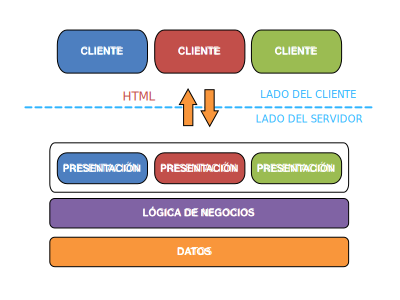
\includegraphics[]{figures/web_arch.png}
	\caption{Arquitectura em capas básica de un sistema web.}
	\label{fig:intro:jvm:web_arch}
\end{figure}
 
\subsection{Reutilización de código mediante \dependencies}
\label{subsec:intro:jvm_dev:dependencies}

Existen numerosos \frameworks, \toolkits, bibliotecas y porciones de código 
que los desarrolladores pueden utilizar en el código de su proyecto para 
obtener funcionalidades genéricas previamente desarrolladas. Estas porciones 
de código de terceros reciben el nombre de \dependencies.\\
En éste trabajo se identificaran dos tipos de \dependencies: las de la 
\logictier, dadas por \emph{paquetes} de código \java compilado (archivos 
.jar\footnote{
	.jar es una extensión de archivo utilizada por aplicaciones de la 
	plataforma \java. Es un archivo comprimido que contiene en su interior
	código \bytecode \java junto con metadata. Son, básicamente, programas que
	corren en la \jvm.
} 
o .war\footnote{
	.war es una extensión de archivo utilizada por aplicaciones de la 
	plataforma \java que corren en servidores web.
}), y las de \viewtier que consisten en (pero no se limitan a) archivos 
\css y \js. A su vez, dichas \dependencies pueden ser manejadas o no 
manejadas.\\
Las \dependencies no manejadas son código que se agrega manualmente al
proyecto mediante la clásica técnica de \quoted{copiar y pegar} o agregando los 
archivos correspondientes a esa \dependency en una carpeta del proyecto 
(proceso que se denominará \quoted{instalar}). Por su parte, las \dependencies 
manejadas consisten en algún \conffile que describe inequívocamente 
(generalmente mediante el nombre y la versión) las \dependencies de terceros 
requeridas en el código a desarrollar. Un programa externo evaluará el 
\conffile al momento de la compilación y se encargará de descargar e 
\emph{instalar} las \dependencies declaradas. Estos programas son conocidos 
como \depmgrs. La \figref{fig:intro:jvm:dep_types} muestra los tipos de \dependencies.

\begin{figure}[tb]
	\centering
	\includegraphics[]{figures/dep_types.png}
	\caption{Distintos tipos de \dependencies.}
	\label{fig:intro:jvm:dep_types}
\end{figure}

Las \dependencies no manejadas implican una serie de pasos repetitivos y 
propensos a errores que el usuario debe realizar para correr su código. Por su 
parte, las \dependencies manejadas son preferentes, ya que eliminan errores 
comunes y ahorran tiempo y trabajo a los desarrolladores. Además, los \depmgrs 
suelen simplificar la complejidad asociada a instalar las \dependencies 
anidadas\footnote{
	Asuma el lector un proyecto \emph{A} con una \dependency \emph{B}. El 
	paquete \emph{B} es a su vez un proyecto con \dependencies, por ejemplo 
	\emph{C}. Para que \emph{A} funcione correctamente, requiere \emph{B} y 
	este a su vez requiere \emph{C}, haciendo que de forma transitiva \emph{A} 
	requiera \emph{C}.
} \citesq{Larman:2010:BOOK}.\\
Las \dependencies de la \viewtier en la plataforma \java, suelen ser no 
manejadas. El presente trabajo se enfoca en transformar esas \dependencies, en 
\dependencies manejadas.\\

\jump[1]

El presente trabajo tratará la implementación de un \depmgrs para descargar 
librerías web (archivos \css, \js, y otros) en sistemas que compilan a 
\bytecode \java. Para hacer un \depmgr de la \viewtier se utilizarán conceptos 
utilizados por herramientas existentes que trabajan sobre la \logictier, además 
de integrarse con dichas herramientas cuando sea posible.